
\chapter{One Sample Confidence Intervals on a Mean When the Population Variance is Known}
\section{Introduction}
Statistical inference is concerned primarily with understanding the quality of parameter estimates. For example, a classic inferential question is, ``How sure are we that the estimated mean, $\bar{x}$, is near the true population mean, $\mu$?'' While the equations and details change depending on the setting, the foundations for inference are the same throughout all of statistics. We introduce these common themes by discussing inference about the population mean, $\mu$, and set the stage for other parameters and scenarios. Some advanced considerations are discussed. Understanding this chapter will make the rest of this book, and indeed the rest of statistics, seem much more familiar.

\begin{definition}[Key Terms]
\textbf{Population:} A group of interest (typically large). 
\vspace{0.1em}

\textbf{Sample:} A subset of a population. 

\textbf{Parameter (of population):} A numerical characteristic of a population. These are usually \textcolor{blue}{unknown} in real-life settings. \\
\hspace*{1em} $\mu$: population mean \\
\hspace*{1em} $\sigma^2$: population variance \\
\hspace*{1em} $\sigma$: population standard deviation \\
\textcolor{blue}{Note: Different from a parameter of a distribution.} 

\textbf{Statistic (of sample):} A numerical characteristic of a sample, which is calculated and known (i.e., a function of the data). \\
\hspace*{1em} $\bar{x}$: sample mean \\
\hspace*{1em} $s^2$: sample variance \\
\hspace*{1em} $s$: sample standard deviation \\

\textbf{Statistical Inference:} Use statistics (known) to make conclusions on parameters (unknown) and quantify the degree of certainty of statements made.

\end{definition}
\noindent
The sample mean, $\bar{x} = \frac{1}{n} \sum_{i=1}^{n} x_i$, is a number we use to estimate the population mean, $\mu$. This is called a \textbf{point estimate}. % one value, single best estimate of a parameter

\vspace{1em}

But, we know it’s not equal to $\mu$. Then, we’d rather estimate the population mean using an \textbf{interval estimate} that gives a \textit{range of real numbers} that we hope contains the population mean, $\mu$.
\vspace{1em}
\begin{example}

\begin{itemize}
    \item $\bar{x}$ is a point estimate of $\mu$
    \item $s^2$ is a point estimate of $\sigma^2$
    \item $s$ is a point estimate of $\sigma$
\end{itemize}

\vspace{0.5em}
\textcolor{blue}{\textit{(All calculated with data from a sample)}}

\end{example}

Due to the nature of randomness and calculating based on a subset, statistics are not guaranteed to be exactly equal to parameters.

\vspace{1em}

Therefore, we create \underline{intervals} around statistics which we believe capture the parameter.

\vspace{0.5em}

\noindent
\begin{definition}[Confidence Interval]
A confidence interval is a plausible range of values that captures a parameter with a quantified degree of confidence.
\end{definition}



\vspace{1em}

\begin{figure}[h]
\centering
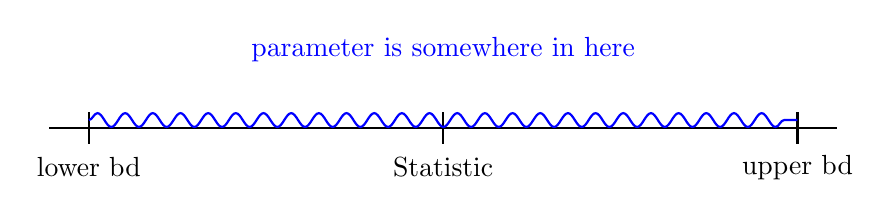
\begin{tikzpicture}
    \draw[thick] (-5,0) -- (5,0);
    \draw[thick] (-4.5,0.2) -- (-4.5,-0.2); % lower bd
    \draw[thick] (0,0.2) -- (0,-0.2);       % statistic
    \draw[thick] (4.5,0.2) -- (4.5,-0.2);   % upper bd
    \node at (-4.5,-0.5) {lower bd};
    \node at (0,-0.5) {Statistic};
    \node at (4.5,-0.5) {upper bd};
    \node[blue] at (0,1) {parameter is somewhere in here};
    \draw[blue, thick, decorate, decoration={snake}] (-4.5,0.1) -- (4.5,0.1);
\end{tikzpicture}
\vspace{-0.5em} % adjust this negative space to reduce space
\caption{Parameter location within the interval.}
\end{figure}

\vspace{2em}
Suppose we are interested in the average mark for \texttt{STA258} for the current semester. We are 100\% confident that the average mark is between 0 and 100; however, this is not useful information as we already know that the average mark must lie between 0 and 100. Using the marks of previous years, we can construct a 95\% interval for the average mark. If it is determined that the average mark lies within 70\% and 80\%, this is much more meaningful as we can state with a high degree of certainty that the average mark is going to lie within a substantially narrow range.


\noindent
\vspace{0.5em}
In this course, all confidence intervals have the same basic skeleton:

\begin{tcolorbox}[
    colback=yellow!10, 
    colframe=black!80, 
    sharp corners=south, 
    boxrule=0.5pt,
    breakable,
    enhanced
]
\[
\textit{estimator} \pm 
\underbrace{
\left(
\textit{value from reference distribution}
\right)
\times 
\left(
\textit{standard error of estimate}
\right)
}_{\text{\textit{margin of error}}}
\]
\end{tcolorbox}

The value from the reference distribution in the skeleton above will be either a value from the standard normal distribution or the Student \textit{t}-distribution. The margin of error (\textit{MOE}) can be considered as the distance around our estimator in which the true value of the parameter of interest will be found, with a specified level of confidence.

\vspace{1em}

\begin{figure}[H]
\label{figureVisualization of CI}
\begin{center}
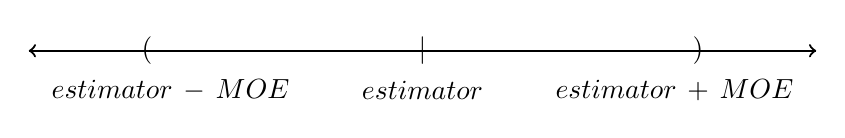
\begin{tikzpicture}
\draw[thick, ->] (-5,0) -- (5,0);
\draw[thick, <-] (-5,0) -- (5,0);
\node at (-3.5,0) {(};
\node at (0,0) {$|$};
\node at (3.5,0) {)};
\node at (0,-0.5) {$estimator$};
\node at (-3.2,-0.5) {$estimator \, - \, MOE$};
\node at (3.2,-0.5) {$estimator \, + \, MOE$};
\end{tikzpicture}
\end{center}
\vspace{-0.60cm}
\caption{Visualization of a confidence interval on the real number line. The margin of error is abbreviated as $MOE$. The estimator is the centre of the interval. The confidence interval consists of all values between the estimator$- MOE$ and the estimator$+ MOE$.}
\end{figure}

\section{Interpretation}

We use very specific language when we interpret a confidence interval.

\begin{tcolorbox}[
    colback=yellow!10, 
    colframe=black!80, 
    sharp corners=south, 
    boxrule=0.5pt,
    breakable,
    enhanced
]
\textit{Suppose we construct a $C\%$ confidence interval for some parameter such that $C$ is between 0 and 100. In repeated sampling, we are $C\%$ confident that approximately $C\%$ of the intervals will capture the true value of the parameter.}
\end{tcolorbox}

\bigskip

By this we mean that if we constructed several $C\%$ confidence intervals using different samples (with or without replacing the units), then we should expect approximately $C\%$ of these intervals to capture the parameter of interest. For example suppose we construct 1000 95\% confidence intervals for the population mean $\mu$. We would expect approximately 95\% of these 1000 intervals (i.e.\ $95\% \times 1000 = 950$) to actually capture $\mu$.



\begin{nt}
A more intuitive but equivalent interpretation is to state that we are $C$\% confident that our target parameter is inside the interval constructed.
\end{nt}

It is incorrect to state that there is a $C\%$ probability that 
the interval we constructed contains the parameter of interest.
We assume that the value of a parameter is fixed. Therefore when we construct a confidence interval, the interval either contains the parameter or it does not.
\section{Confidence Interval for $\mu$ (Known Variance)}
When we know the population standard deviation $\sigma$, we can construct a confidence interval for $\mu$ in the following manner.

\begin{tcolorbox}[
    colback=yellow!10, 
    colframe=black!45, 
    sharp corners=south, 
    boxrule=0.5pt,
    breakable,
    enhanced,
    title={\textbf{Confidence Interval 6.1} (Confidence Interval on $\mu$ when $\sigma$ is Known)}
]

\textit{A $(100 - \alpha)\%$ confidence interval on $\mu$ when $\sigma$ is known is}
\[
\bar{x} \; \pm \; z_{\alpha/2} \left( \frac{\sigma}{\sqrt{n}} \right)
\]

\end{tcolorbox}

The $z_{\alpha/2}$ value is obtained from standard normal tables. The standard error is $\frac{\sigma}{\sqrt{n}}$ and the margin of error is $z_{\alpha/2} \left( \frac{\sigma}{\sqrt{n}} \right)$.
\vspace{0.5em} \\
Let $X_1, X_2, ..., X_n$ be iid $N(\mu, \sigma^2)$, where $\mu$ is unknown and $\sigma$ is known.

We know that:
\[
Z = \frac{\bar{X} - \mu}{\sigma / \sqrt{n}} \sim N(0, 1)
\]
and
\[
P(-1.96 < Z < 1.96) = 0.95
\]
Therefore:
\[
P\left( -1.96 < \frac{\bar{X} - \mu}{\sigma / \sqrt{n}} < 1.96 \right) = 0.95
\Rightarrow P\left( \bar{X} - 1.96 \frac{\sigma}{\sqrt{n}} < \mu < \bar{X} + 1.96 \frac{\sigma}{\sqrt{n}} \right) = 0.95
\]

\vspace{1.5em}
\textbf{Interpretation of Confidence Interval:}

\begin{itemize}
  \item This is a random interval $\bar{X} \pm 1.96 \frac{\sigma}{\sqrt{n}}$
  \item The interval is random since $\bar{X}$ is random due to sampling.
  \item The population mean $\mu$ is a fixed, but unknown, number.
  \item The probability $\mu$ is inside the random interval is 0.95 (success rate of the method).
  \item 95\% of all samples give an interval that captures $\mu$, and 5\% do not.
\end{itemize}

\vspace{1em}
Once we observe our sample:

\begin{itemize}
  \item This is \textbf{not} a random interval $\bar{X} \pm 1.96 \frac{\sigma}{\sqrt{n}}$
  \item The probability $\mu$ is inside this interval is either 1 or 0
\end{itemize}

\vspace{1em}
\textbf{Confidence Interval Isn’t Always Right:}

Not all CIs contain the true value of the parameter. This can be illustrated by plotting many intervals simultaneously and observing.


\vspace{2em}
\textbf{R Output:}
\begin{tcolorbox}[colback=gray!10, colframe=black!45, arc=2mm]
\begin{verbatim}
## Step 1. Generate random samples;
set.seed(2017)
m = 50;       # m = number of samples;
n = 25;       # n = number of obs in sample;
mu.i = 0;     # mu.i = mean of obs;
sigma.i = 5;  # sigma.i = std. dev. of obs;

mu.total = n * mu.i;          # mean of Total;
sigma.total = sqrt(n) * sigma.i;  # std. dev. of Total;
\end{verbatim}
\end{tcolorbox}

\vspace{1em}
\begin{tcolorbox}[colback=gray!10, colframe=black!45, arc=2mm]
\begin{verbatim}
## Step 2. Construct CIs;
xbar = rnorm(m, mu.total, sigma.total) / n;
SE = sigma.i / sqrt(n);

alpha = 0.10;
z.star = qnorm(1 - alpha / 2);
\end{verbatim}
\end{tcolorbox}

\vspace{1em}
\begin{tcolorbox}[colback=gray!10, colframe=black!45, arc=2mm]
\begin{verbatim}
## Step 3. Graph CIs;
matplot(rbind(xbar - z.star * SE, xbar + z.star * SE),
        rbind(1:m, 1:m),
        type = "l", lty = 1,
        xlab = " ", lab = " ");
abline(v = 0, lty = 2);
\end{verbatim}
\end{tcolorbox}

\begin{figure}[H]
  \centering
  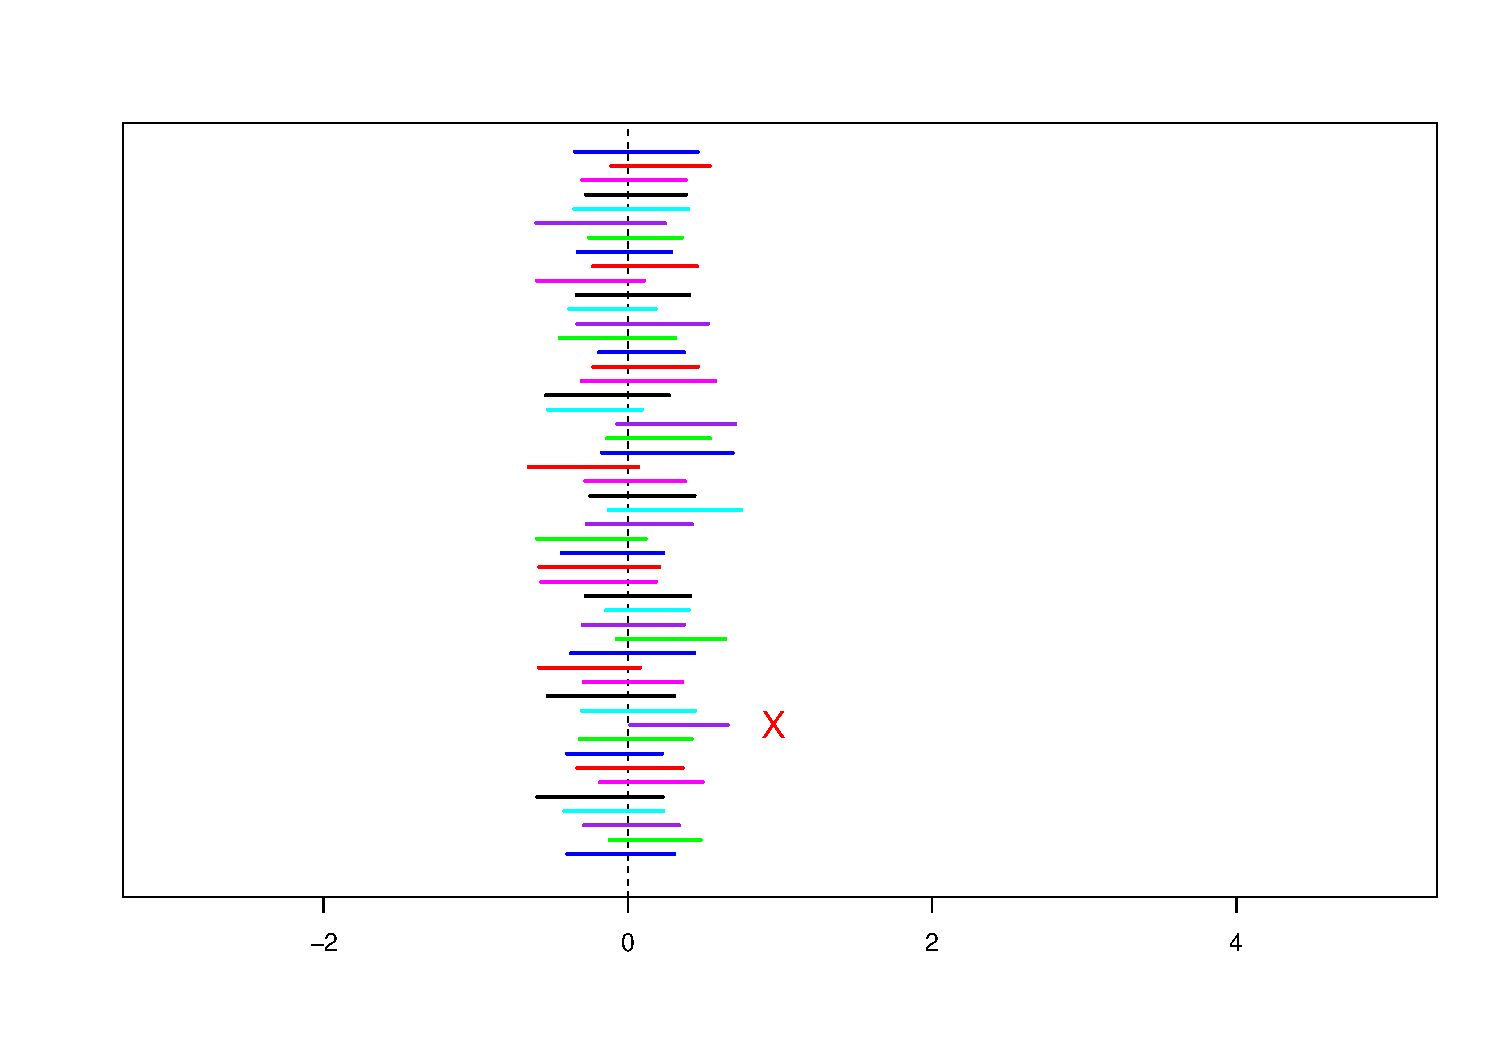
\includegraphics[width=0.6\textwidth]{Section6/images/confidence_intervals.pdf}
\captionsetup{skip=-5pt}
  \caption{Simulated 95\% confidence intervals for the population mean. Red “X” marks indicate intervals that do not contain the true mean (\( \mu = 0 \)).}
\end{figure}


\vspace{2em}

\section*{Confidence Interval for the Mean of a Normal Population}

Draw an SRS (Simple Random Sample) of size $n$ from a Normal population having unknown mean $\mu$ and \textbf{known} standard deviation $\sigma$. A level $C$ confidence interval for $\mu$ is:

\[
\bar{x} \pm z_{\ast} \cdot \frac{\sigma}{\sqrt{n}}
\]

The critical value $z_{\ast}$ is illustrated in a Figure below and depends on $C$.

\begin{figure}[H]
  \centering
  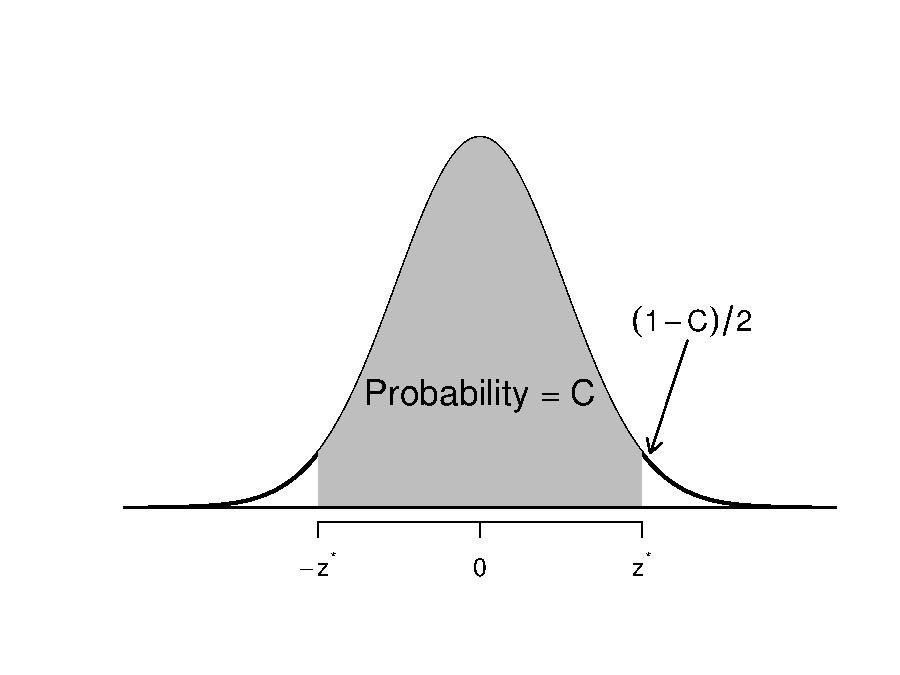
\includegraphics[width=0.6\textwidth]{Section6/images/normal_confidence_curve.pdf}
\vspace{-0.7em} % Adjust this negative space to decrease gap; you can change -0.7em to a suitable value
\captionsetup{skip=0pt} % remove vertical space above caption
 \caption{The central area under the standard normal curve with confidence level \( C \).}
\end{figure}

\section*{Large Sample CI for $\mu$ (Normal data)}
When we have a large sample from a Normal distribution, the confidence interval for the population mean \(\mu\) can be approximated by the formula:
\[
\bar{x} \pm z_{\alpha/2} \cdot \frac{\sigma}{\sqrt{n}}
\]

This formula is valid under the following assumptions:
\begin{itemize}
  \item $n$ large
  \item random sample from a Normal distribution
  \item independent observations
\end{itemize}

Some definitions:
\begin{itemize}
  \item $1 - \alpha$ is the confidence coefficient
  \item $100(1 - \alpha)\%$ is the confidence level
\end{itemize}


\section*{One Sample CI on the Population Mean $\mu$}
To construct a confidence interval for the population mean, we rely on several important assumptions:
\begin{itemize}
  \item When population standard deviation $\sigma$ is \textbf{known}
  \item Formula: $\bar{x} \pm z_{\alpha/2} \cdot \frac{\sigma}{\sqrt{n}}$
  \item Margin of error comes from standard normal and standard error
\end{itemize}

How to find $z_{\alpha/2}$?

Example: Find $z_{\alpha/2}$ for a 95\% CI on $\mu$:
\[
1 - \alpha = 0.95, \quad \alpha = 0.05, \quad \alpha/2 = 0.025
\]
\[
z_{\alpha/2} = 1.96 \quad (\text{from table or R: } \texttt{qnorm(0.975)})
\]


\section*{Table of Common $z$-values}

\begin{center}
\begin{tabular}{|c|c|c|}
\hline
Confidence coefficient & Confidence level & $z$ \\
\hline
0.90 & 90\% & 1.645 \\
0.95 & 95\% & 1.96 \\
0.99 & 99\% & 2.576 \\
\hline
\end{tabular}
\end{center}



\begin{example}
Playbill magazine reported that the mean annual household income of its readers is \$119{,}155. Assume this estimate is based on a sample of 80 households, and that the population standard deviation is known to be $\sigma = 30{,}000$.

\begin{itemize}
  \item $\bar{x} = 119{,}155$
  \item $n = 80$
  \item $\sigma = 30{,}000$
\end{itemize}

\textbf{Tasks:}
\begin{enumerate}
  \item[(a)] Develop a 90\% confidence interval estimate of the population mean.
  \item[(b)] Develop a 95\% confidence interval estimate of the population mean.
  \item[(c)] Develop a 99\% confidence interval estimate of the population mean.
\end{enumerate}



\textbf{90\% CI Calculation}

\[
\bar{x} \pm z_{\alpha/2} \cdot \frac{\sigma}{\sqrt{n}} = 119{,}155 \pm 1.645 \cdot \frac{30{,}000}{\sqrt{80}}
\]
\[
= 119{,}155 \pm 5{,}500.73
\]
\[
= (113{,}654.27, \; 124{,}655.73)
\]

\textbf{95\% CI Calculation}

\[
\bar{x} \pm z_{\alpha/2} \cdot \frac{\sigma}{\sqrt{n}} = 119{,}155 \pm 1.96 \cdot \frac{30{,}000}{\sqrt{80}}
\]
\[
= 119{,}155 \pm 6{,}574.04
\]
\[
= (112{,}580.96, \; 125{,}729.04)
\]


\textbf{99\% CI Calculation}

\[
\bar{x} \pm z_{\alpha/2} \cdot \frac{\sigma}{\sqrt{n}} = 119{,}155 \pm 2.576 \cdot \frac{30{,}000}{\sqrt{80}}
\]
\[
= 119{,}155 \pm 8{,}620.04
\]
\[
= (110{,}534.96, \; 127{,}775.04)
\]


\textbf{Interpretation}


We are 99\% confident the mean household income of magazine readers is between \$110{,}534.96 and \$127{,}775.04.
\end{example}
\begin{example}

\vspace{1em}

\noindent\textbf{Scenario:}

\vspace{0.5em}

The number of cars sold annually by used car salespeople is known to be \textbf{normally distributed}, with a population standard deviation of $\sigma = 15$. A random sample of $n = 15$ salespeople was taken, and the number of cars each sold is recorded below. Construct a \textbf{95\% confidence interval} for the population mean number of cars sold, and provide an interpretation.

\vspace{1em}

\noindent\textbf{Raw data:}

\[
\begin{matrix}
79 & 43 & 58 & 66 & 101 \\
63 & 79 & 33 & 58 & 71 \\
60 & 101 & 74 & 55 & 88 \\
\end{matrix}
\]

\vspace{0.5em}

\noindent The sample mean is:

\[
\bar{x} = \frac{79 + 43 + \cdots + 55 + 88}{15} = 68.6
\]

\vspace{1em}

\noindent\textbf{R function:}

\begin{tcolorbox}[colback=gray!10, colframe=gray!50, arc=2mm]
\begin{verbatim}
simple.z.test = function(x, sigma, conf.level = 0.95) {
  n = length(x);
  xbar = mean(x);
  alpha = 1 - conf.level;
  zstar = qnorm(1 - alpha/2);
  SE = sigma / sqrt(n);
  xbar + c(-zstar * SE, zstar * SE);
}
\end{verbatim}
\end{tcolorbox}

\vspace{0.5em}

\noindent\textbf{R output:}

\begin{tcolorbox}[colback=gray!10, colframe=black!45, arc=2mm]
\begin{verbatim}
# Step 1. Entering data;
cars = c(79, 43, 58, 66, 101, 63, 79,
         33, 58, 71, 60, 101, 74, 55, 88)

# Step 2. Finding CI;
simple.z.test(cars, 15)

## [1] 61.00909 76.19091
\end{verbatim}
\end{tcolorbox}

\vspace{1em}

\noindent\textbf{Interpretation:} \textbf{We estimate that the mean number of cars sold annually by all used car salespeople lies between 61 and 76, approximately. This type of estimate is correct 95\% of the time.}

\end{example}

\begin{tcolorbox}[colback=blue!5!white, colframe=blue!75!black,
  title=\textbf{Cases Where Valid}, fonttitle=\bfseries,
  coltitle=white, colbacktitle=blue!90!black, arc=2mm]

\begin{itemize}
  \item Large samples where population is \textbf{normal}.
  \item Large samples where population is \textbf{not normal} (By CLT).
  \item Small samples where population is \textbf{normal}.
\end{itemize}

\textit{Note: A sample is considered large if $n \geq 30$.}
\end{tcolorbox}

\begin{example}
Suppose a student measuring the boiling temperature of a certain liquid observes the readings (in degrees Celsius) 102.5, 101.7, 103.1, 100.9, 100.5, and 102.2 on 6 different samples of the liquid. He calculates the sample mean to be 101.82. If he knows that the distribution of boiling points is Normal, with standard deviation 1.2 degrees, what is the confidence interval for the population mean at a 95\% confidence level?\\
\end{example}
\textbf{A confidence interval} uses sample data to estimate an unknown population parameter with an indication of how accurate the estimate is and of how confident we are that the result is correct.

\vspace{1em}

The \textbf{interval} often has the form\\
\hspace*{2em}estimate $\pm$ margin of error

\vspace{1em}

The \textbf{confidence level} is the success rate of the method that produces the interval.
 A level $C$ \textbf{confidence interval for the mean} $\mu$ of a Normal population with \textbf{known} standard deviation $\sigma$, based on an SRS of size $n$, is given by
\[
\bar{x} \pm z^\star \frac{\sigma}{\sqrt{n}}
\]

The \textbf{critical value} $z^\star$ is chosen so that the standard Normal curve has area $C$ between $-z^\star$ and $z^\star$. \\

Other things being equal, the \textbf{margin of error} of a confidence interval gets smaller as
\begin{itemize}
    \item the confidence level $C$ decreases,
    \item the population standard deviation $\sigma$ decreases, and
    \item the sample size $n$ increases.
\end{itemize}
\vspace{\baselineskip} 
\section{APPENDIX}


Interval estimators are commonly called \textbf{confidence intervals}. The upper and lower endpoints of a confidence interval are called the \textbf{upper} and \textbf{lower confidence limits}, respectively. The probability that a (random) confidence interval will enclose $\theta$ (a fixed quantity) is called the \textbf{confidence coefficient}.\\


Suppose that $\hat{\theta}_L$ and $\hat{\theta}_U$ are the (random) lower and upper confidence limits, respectively, for a parameter $\theta$. Then, if
$$P(\hat{\theta}_L \leq \theta \leq \hat{\theta}_U) = 1 - \alpha,$$
the probability $(1 - \alpha)$ is the \textbf{confidence coefficient}.

\subsection*{Pivotal quantities}
One very useful method for finding confidence intervals is called the \textbf{pivotal method}. This method depends on finding a pivotal quantity that possesses two characteristics:
\begin{itemize}
    \item It is a function of the sample measurements and the unknown parameter $\theta$, where $\theta$ is the \textbf{only} unknown quantity.
    \item Its probability distribution does not depend on the parameter $\theta$.
\end{itemize}


